%
% $Id: $
%
%
% Compilar a .pdf con LaTeX (pdflatex)
% Es necesario instalar Beamer (paquete latex-beamer en Debian)
%

%
% Gr�ficos:
% Los gr�ficos pueden suministrarse en PNG, JPG, TIF, PDF, MPS
% Los EPS deben convertirse a PDF (usar epstopdf)
%

\documentclass{beamer}
\usetheme{GSyC}
%\usebackgroundtemplate{\includegraphics[width=\paperwidth]{format/libresoft-bg.png}}
%\usepackage[spanish]{babel}
\usepackage[latin1]{inputenc}
\usepackage{graphics}
\usepackage{amssymb} % Simbolos matematicos

\ProcessOptions

%% Metadatos del PDF.
\hypersetup{
  pdftitle={Protocolos para la Transmisi�n de Audio y V�deo por Internet},
  pdfauthor={Gregorio Robles, Jes�s M. Gonz�lez Barahona},
  pdfcreator={GSyC, Universidad Rey Juan Carlos},
  pdfproducer=PDFLaTeX,
  pdfsubject={Protocolos para la Transmisi�n de Audio y V�deo por Internet},
}
%%

\begin{document}

\title{Google Cardboard}
\subtitle{Protocolos para la Transmisi�n de Audio y V�deo en Internet}
\institute{\{grex,jgb\}@gsyc.urjc.es \\
GSyC, Universidad Rey Juan Carlos}
\author[Gregorio Robles, Jes�s M. Gonz�lez Barahona]{Gregorio Robles, Jes�s M. Gonz�lez Barahona}
\date[Sept 2014]{9 de septiembre de 2014}


\frame{
\maketitle
}


% Si el titulo o el autor se quieren acortar para los pies de p�gina
% se pueden redefinir aqu�:
%\title{Titulo corto}
%\author{Autores abreviado}


%% LICENCIA DE REDISTRIBUCION DE LAS TRANSPAS
\frame{
~
\vspace{4cm}

\begin{flushright}

\includegraphics[width=2.2cm]{figs/by-sa}

{\tiny
(cc) 2014 Gregorio Robles, Jes�s M. Gonz�lez Barahona \\
  Some rights reserved. This work licensed under Creative Commons \\
  Attribution-ShareAlike License. To view a copy of full license, see \\
\ \\
  http://creativecommons.org/licenses/by-sa/3.0/ or write to \\
  Creative Commons, 559 Nathan Abbott Way, Stanford, \\
  California 94305, USA. \\
\ 
}
\end{flushright}
}
%%


%-----------------------    ---------------------------------

\begin{frame}
\frametitle{Google Cardboard}

\begin{center}
  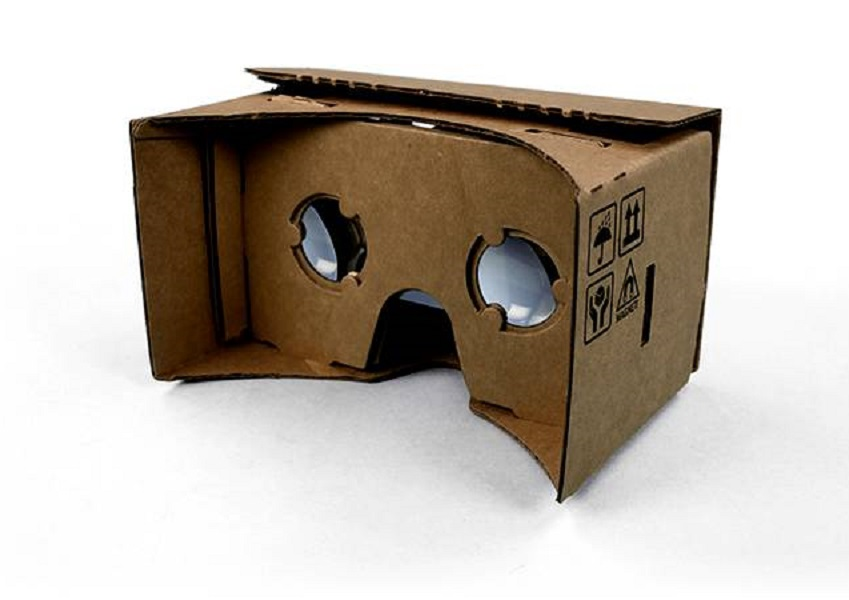
\includegraphics[width=9cm]{figs/google-cardboard.jpg}
\end{center}


\begin{flushright}
{\tiny
Source: http://images.techtimes.com/data/images/full/10137/google-cardboard.jpg
}
\end{flushright}

\end{frame}


%-----------------------    ---------------------------------

\begin{frame}
\frametitle{Google Cardboard}

\begin{center}
  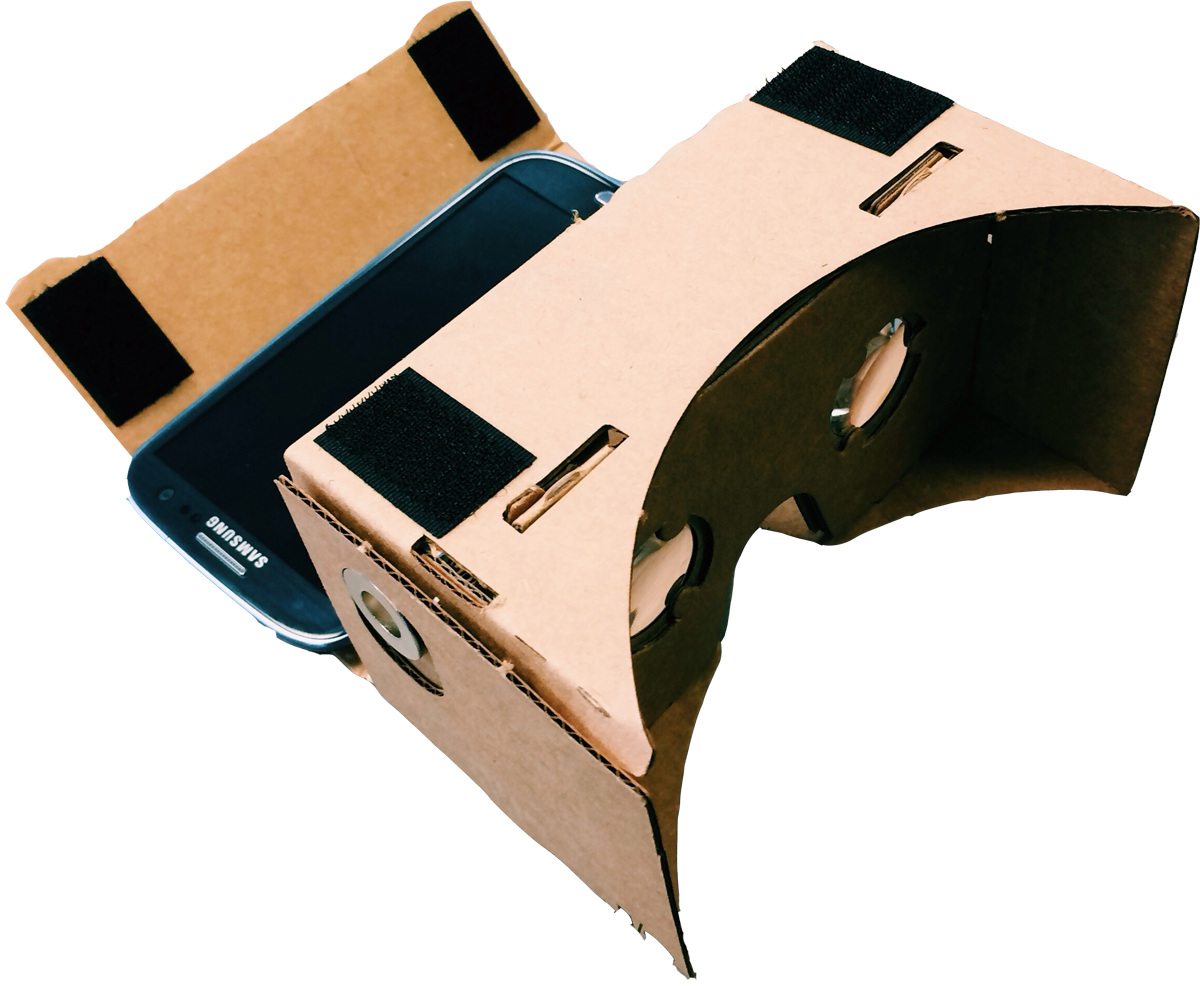
\includegraphics[width=8cm]{figs/google-cardboard2.jpg}
\end{center}


\begin{flushright}
{\tiny
Source: http://uploads.webflow.com/53acec028f16901b3d5ca6c1/53acec104f02f4e04bcd4ec5\_1.png
}
\end{flushright}

\end{frame}


%-----------------------    ---------------------------------

\begin{frame}
\frametitle{�Qu� es el Google Cardboard?}

\begin{itemize}
   \item Experimenta realidad virtual de manera sencilla y barata (19 euros)
   \item Cuesta 35\% (aunque hay instrucciones para hacerla t� mismo con una caja de pizza)
   \item Hay varias aplicaciones en el Google Play: cardboard, etc.
   \item API en Java
   \item Tambi�n se pueden utilizar extensiones de Chrome escritas en Javascript (con Tree.js)
\end{itemize}

\end{frame}


%-----------------------    ---------------------------------

\begin{frame}
\frametitle{Google Cardboard ``ingredients''}

\begin{center}
  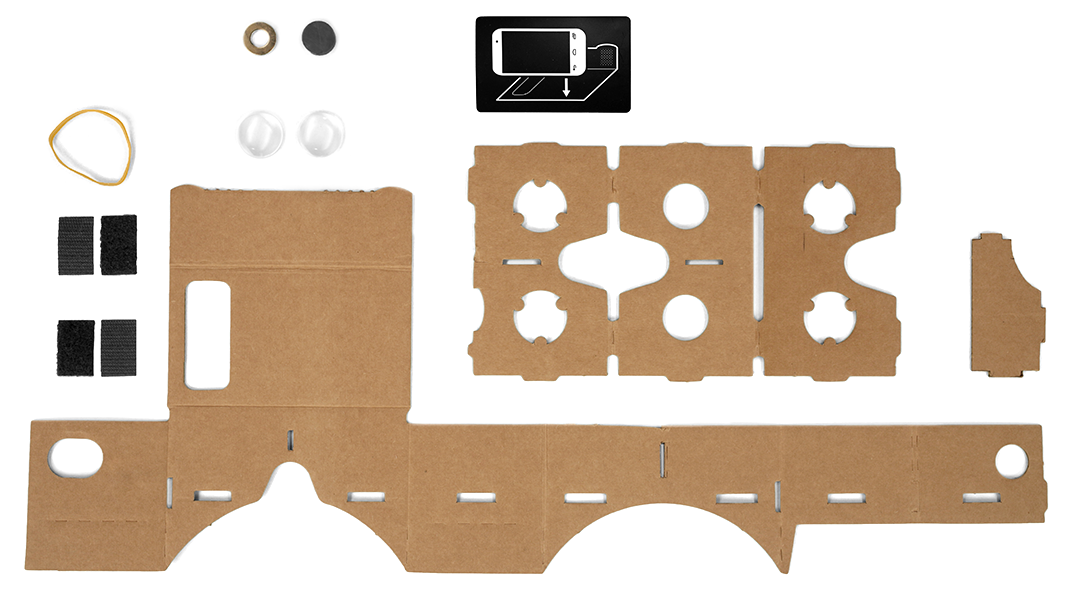
\includegraphics[width=11cm]{figs/ingredients.png}
\end{center}


\begin{flushright}
{\tiny
Source: https://cardboard.withgoogle.com/
}
\end{flushright}

\end{frame}


\frame{
\maketitle
}

\end{document}
